\chapter{The King’s Closet at the Tuileries}

We will leave Villefort on the road to Paris, travelling—thanks to
trebled fees—with all speed, and passing through two or three
apartments, enter at the Tuileries the little room with the arched
window, so well known as having been the favorite closet of Napoleon
and Louis XVIII., and now of Louis Philippe.

There, seated before a walnut table he had brought with him from
Hartwell, and to which, from one of those fancies not uncommon to great
people, he was particularly attached, the king, Louis XVIII., was
carelessly listening to a man of fifty or fifty-two years of age, with
gray hair, aristocratic bearing, and exceedingly gentlemanly attire,
and meanwhile making a marginal note in a volume of Gryphius’s rather
inaccurate, but much sought-after, edition of Horace—a work which was
much indebted to the sagacious observations of the philosophical
monarch.

“You say, sir——” said the king.

“That I am exceedingly disquieted, sire.”

“Really, have you had a vision of the seven fat kine and the seven lean
kine?”

“No, sire, for that would only betoken for us seven years of plenty and
seven years of scarcity; and with a king as full of foresight as your
majesty, scarcity is not a thing to be feared.”

“Then of what other scourge are you afraid, my dear Blacas?”

“Sire, I have every reason to believe that a storm is brewing in the
south.”

“Well, my dear duke,” replied Louis XVIII., “I think you are wrongly
informed, and know positively that, on the contrary, it is very fine
weather in that direction.” Man of ability as he was, Louis XVIII.
liked a pleasant jest.

“Sire,” continued M. de Blacas, “if it only be to reassure a faithful
servant, will your majesty send into Languedoc, Provence, and Dauphiné,
trusty men, who will bring you back a faithful report as to the feeling
in these three provinces?”

“\textit{Canimus surdis},” replied the king, continuing the annotations in his
Horace.

“Sire,” replied the courtier, laughing, in order that he might seem to
comprehend the quotation, “your majesty may be perfectly right in
relying on the good feeling of France, but I fear I am not altogether
wrong in dreading some desperate attempt.”

“By whom?”

“By Bonaparte, or, at least, by his adherents.”

“My dear Blacas,” said the king, “you with your alarms prevent me from
working.”

“And you, sire, prevent me from sleeping with your security.”

“Wait, my dear sir, wait a moment; for I have such a delightful note on
the \textit{Pastor quum traheret}—wait, and I will listen to you afterwards.”

There was a brief pause, during which Louis XVIII. wrote, in a hand as
small as possible, another note on the margin of his Horace, and then
looking at the duke with the air of a man who thinks he has an idea of
his own, while he is only commenting upon the idea of another, said:

“Go on, my dear duke, go on—I listen.”

“Sire,” said Blacas, who had for a moment the hope of sacrificing
Villefort to his own profit, “I am compelled to tell you that these are
not mere rumors destitute of foundation which thus disquiet me; but a
serious-minded man, deserving all my confidence, and charged by me to
watch over the south” (the duke hesitated as he pronounced these
words), “has arrived by post to tell me that a great peril threatens
the king, and so I hastened to you, sire.”

“\textit{Mala ducis avi domum},” continued Louis XVIII., still annotating.

“Does your majesty wish me to drop the subject?”

“By no means, my dear duke; but just stretch out your hand.”

“Which?”

“Whichever you please—there to the left.”

“Here, sire?”

“I tell you to the left, and you are looking to the right; I mean on my
left—yes, there. You will find yesterday’s report of the minister of
police. But here is M. Dandré himself;” and M. Dandré, announced by the
chamberlain-in-waiting, entered.

“Come in,” said Louis XVIII., with repressed smile, “come in, Baron,
and tell the duke all you know—the latest news of M. de Bonaparte; do
not conceal anything, however serious,—let us see, the Island of Elba
is a volcano, and we may expect to have issuing thence flaming and
bristling war—\textit{bella, horrida bella}.”

M. Dandré leaned very respectfully on the back of a chair with his two
hands, and said:

“Has your majesty perused yesterday’s report?”

“Yes, yes; but tell the duke himself, who cannot find anything, what
the report contains—give him the particulars of what the usurper is
doing in his islet.”

“Monsieur,” said the baron to the duke, “all the servants of his
majesty must approve of the latest intelligence which we have from the
Island of Elba. Bonaparte——”

M. Dandré looked at Louis XVIII., who, employed in writing a note, did
not even raise his head. “Bonaparte,” continued the baron, “is mortally
wearied, and passes whole days in watching his miners at work at
Porto-Longone.”

“And scratches himself for amusement,” added the king.

“Scratches himself?” inquired the duke, “what does your majesty mean?”

“Yes, indeed, my dear duke. Did you forget that this great man, this
hero, this demigod, is attacked with a malady of the skin which worries
him to death, \textit{prurigo}?”

“And, moreover, my dear duke,” continued the minister of police, “we
are almost assured that, in a very short time, the usurper will be
insane.”

“Insane?”

“Raving mad; his head becomes weaker. Sometimes he weeps bitterly,
sometimes laughs boisterously, at other time he passes hours on the
seashore, flinging stones in the water and when the flint makes
‘duck-and-drake’ five or six times, he appears as delighted as if he
had gained another Marengo or Austerlitz. Now, you must agree that
these are indubitable symptoms of insanity.”

“Or of wisdom, my dear baron—or of wisdom,” said Louis XVIII.,
laughing; “the greatest captains of antiquity amused themselves by
casting pebbles into the ocean—see Plutarch’s life of Scipio
Africanus.”

M. de Blacas pondered deeply between the confident monarch and the
truthful minister. Villefort, who did not choose to reveal the whole
secret, lest another should reap all the benefit of the disclosure, had
yet communicated enough to cause him the greatest uneasiness.

“Well, well, Dandré,” said Louis XVIII., “Blacas is not yet convinced;
let us proceed, therefore, to the usurper’s conversion.” The minister
of police bowed.

“The usurper’s conversion!” murmured the duke, looking at the king and
Dandré, who spoke alternately, like Virgil’s shepherds. “The usurper
converted!”

“Decidedly, my dear duke.”

“In what way converted?”

“To good principles. Tell him all about it, baron.”

“Why, this is the way of it,” said the minister, with the gravest air
in the world: “Napoleon lately had a review, and as two or three of his
old veterans expressed a desire to return to France, he gave them their
dismissal, and exhorted them to ‘serve the good king.’ These were his
own words, of that I am certain.”

“Well, Blacas, what think you of this?” inquired the king triumphantly,
and pausing for a moment from the voluminous scholiast before him.

“I say, sire, that the minister of police is greatly deceived or I am;
and as it is impossible it can be the minister of police as he has the
guardianship of the safety and honor of your majesty, it is probable
that I am in error. However, sire, if I might advise, your majesty will
interrogate the person of whom I spoke to you, and I will urge your
majesty to do him this honor.”

“Most willingly, duke; under your auspices I will receive any person
you please, but you must not expect me to be too confiding. Baron, have
you any report more recent than this, dated the 20th February, and this
is the 3rd of March?”

“No, sire, but I am hourly expecting one; it may have arrived since I
left my office.”

“Go thither, and if there be none—well, well,” continued Louis XVIII.,
“make one; that is the usual way, is it not?” and the king laughed
facetiously.

“Oh, sire,” replied the minister, “we have no occasion to invent any;
every day our desks are loaded with most circumstantial denunciations,
coming from hosts of people who hope for some return for services which
they seek to render, but cannot; they trust to fortune, and rely upon
some unexpected event in some way to justify their predictions.”

“Well, sir, go,” said Louis XVIII., “and remember that I am waiting for
you.”

“I will but go and return, sire; I shall be back in ten minutes.”

“And I, sire,” said M. de Blacas, “will go and find my messenger.”

“Wait, sir, wait,” said Louis XVIII. “Really, M. de Blacas, I must
change your armorial bearings; I will give you an eagle with
outstretched wings, holding in its claws a prey which tries in vain to
escape, and bearing this device—\textit{Tenax}.”

\begin{figure}[h]
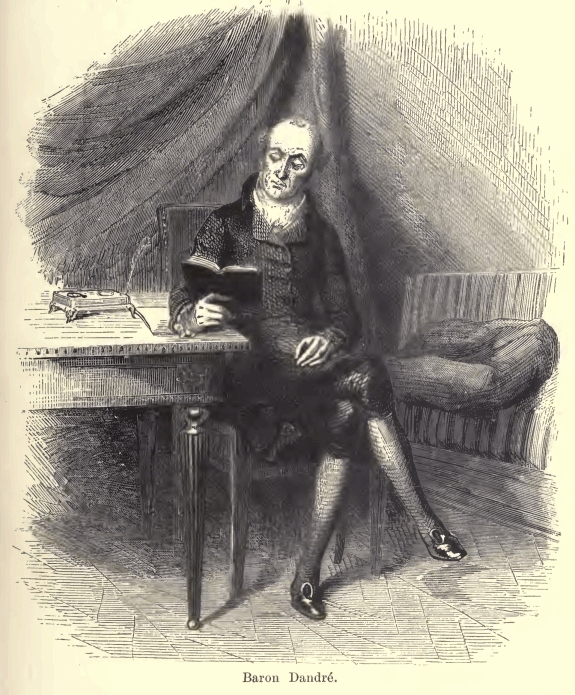
\includegraphics[width=\textwidth]{0133m.jpg}
\end{figure}

“Sire, I listen,” said De Blacas, biting his nails with impatience.

“I wish to consult you on this passage, ‘\textit{Molli fugiens anhelitu},’ you
know it refers to a stag flying from a wolf. Are you not a sportsman
and a great wolf-hunter? Well, then, what do you think of the \textit{molli
anhelitu}?”

“Admirable, sire; but my messenger is like the stag you refer to, for
he has posted two hundred and twenty leagues in scarcely three days.”

“Which is undergoing great fatigue and anxiety, my dear duke, when we
have a telegraph which transmits messages in three or four hours, and
that without getting in the least out of breath.”

“Ah, sire, you recompense but badly this poor young man, who has come
so far, and with so much ardor, to give your majesty useful
information. If only for the sake of M. de Salvieux, who recommends him
to me, I entreat your majesty to receive him graciously.”

“M. de Salvieux, my brother’s chamberlain?”

“Yes, sire.”

“He is at Marseilles.”

“And writes me thence.”

“Does he speak to you of this conspiracy?”

“No; but strongly recommends M. de Villefort, and begs me to present
him to your majesty.”

“M. de Villefort!” cried the king, “is the messenger’s name M. de
Villefort?”

“Yes, sire.”

“And he comes from Marseilles?”

“In person.”

“Why did you not mention his name at once?” replied the king, betraying
some uneasiness.

“Sire, I thought his name was unknown to your majesty.”

“No, no, Blacas; he is a man of strong and elevated understanding,
ambitious, too, and, \textit{pardieu!} you know his father’s name!”

“His father?”

“Yes, Noirtier.”

“Noirtier the Girondin?—Noirtier the senator?”

“He himself.”

“And your majesty has employed the son of such a man?”

“Blacas, my friend, you have but limited comprehension. I told you
Villefort was ambitious, and to attain this ambition Villefort would
sacrifice everything, even his father.”

“Then, sire, may I present him?”

“This instant, duke! Where is he?”

“Waiting below, in my carriage.”

“Seek him at once.”

“I hasten to do so.”

The duke left the royal presence with the speed of a young man; his
really sincere royalism made him youthful again. Louis XVIII. remained
alone, and turning his eyes on his half-opened Horace, muttered:

“\textit{Justum et tenacem propositi virum}.”

M. de Blacas returned as speedily as he had departed, but in the
antechamber he was forced to appeal to the king’s authority.
Villefort’s dusty garb, his costume, which was not of courtly cut,
excited the susceptibility of M. de Brezé, who was all astonishment at
finding that this young man had the audacity to enter before the king
in such attire. The duke, however, overcame all difficulties with a
word—his majesty’s order; and, in spite of the protestations which the
master of ceremonies made for the honor of his office and principles,
Villefort was introduced.

The king was seated in the same place where the duke had left him. On
opening the door, Villefort found himself facing him, and the young
magistrate’s first impulse was to pause.

“Come in, M. de Villefort,” said the king, “come in.”

Villefort bowed, and advancing a few steps, waited until the king
should interrogate him.

“M. de Villefort,” said Louis XVIII., “the Duc de Blacas assures me you
have some interesting information to communicate.”

“Sire, the duke is right, and I believe your majesty will think it
equally important.”

\begin{figure}[h]
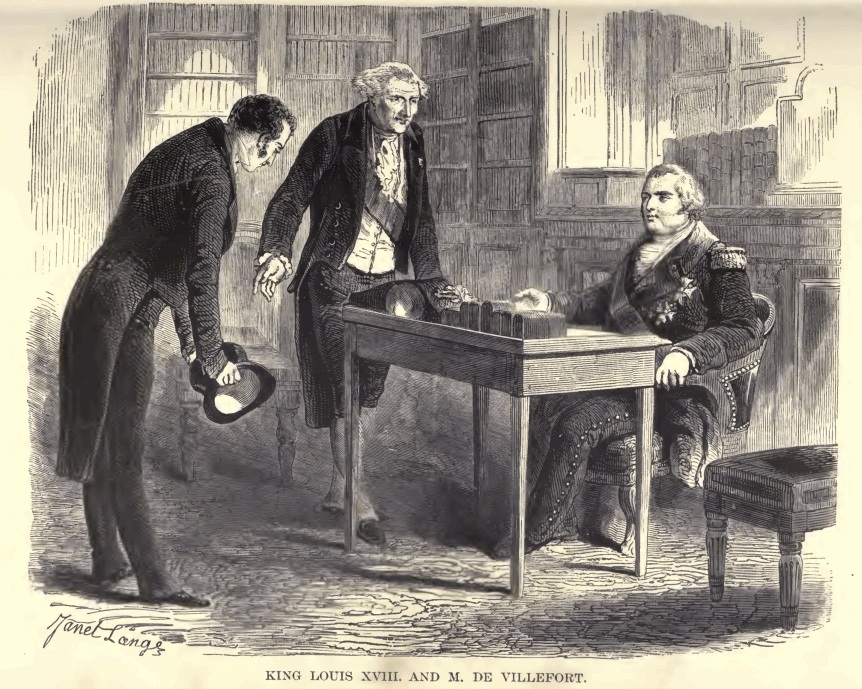
\includegraphics[width=\textwidth]{0137m.jpg}
\end{figure}

“In the first place, and before everything else, sir, is the news as
bad in your opinion as I am asked to believe?”

“Sire, I believe it to be most urgent, but I hope, by the speed I have
used, that it is not irreparable.”

“Speak as fully as you please, sir,” said the king, who began to give
way to the emotion which had showed itself in Blacas’s face and
affected Villefort’s voice. “Speak, sir, and pray begin at the
beginning; I like order in everything.”

“Sire,” said Villefort, “I will render a faithful report to your
majesty, but I must entreat your forgiveness if my anxiety leads to
some obscurity in my language.” A glance at the king after this
discreet and subtle exordium, assured Villefort of the benignity of his
august auditor, and he went on:

“Sire, I have come as rapidly to Paris as possible, to inform your
majesty that I have discovered, in the exercise of my duties, not a
commonplace and insignificant plot, such as is every day got up in the
lower ranks of the people and in the army, but an actual conspiracy—a
storm which menaces no less than your majesty’s throne. Sire, the
usurper is arming three ships, he meditates some project, which,
however mad, is yet, perhaps, terrible. At this moment he will have
left Elba, to go whither I know not, but assuredly to attempt a landing
either at Naples, or on the coast of Tuscany, or perhaps on the shores
of France. Your majesty is well aware that the sovereign of the Island
of Elba has maintained his relations with Italy and France?”

“I am, sir,” said the king, much agitated; “and recently we have had
information that the Bonapartist clubs have had meetings in the Rue
Saint-Jacques. But proceed, I beg of you. How did you obtain these
details?”

“Sire, they are the results of an examination which I have made of a
man of Marseilles, whom I have watched for some time, and arrested on
the day of my departure. This person, a sailor, of turbulent character,
and whom I suspected of Bonapartism, has been secretly to the Island of
Elba. There he saw the grand-marshal, who charged him with an oral
message to a Bonapartist in Paris, whose name I could not extract from
him; but this mission was to prepare men’s minds for a return (it is
the man who says this, sire)—a return which will soon occur.”

“And where is this man?”

“In prison, sire.”

“And the matter seems serious to you?”

“So serious, sire, that when the circumstance surprised me in the midst
of a family festival, on the very day of my betrothal, I left my bride
and friends, postponing everything, that I might hasten to lay at your
majesty’s feet the fears which impressed me, and the assurance of my
devotion.”

“True,” said Louis XVIII., “was there not a marriage engagement between
you and Mademoiselle de Saint-Méran?”

“Daughter of one of your majesty’s most faithful servants.”

“Yes, yes; but let us talk of this plot, M. de Villefort.”

“Sire, I fear it is more than a plot; I fear it is a conspiracy.”

“A conspiracy in these times,” said Louis XVIII., smiling, “is a thing
very easy to meditate, but more difficult to conduct to an end,
inasmuch as, re-established so recently on the throne of our ancestors,
we have our eyes open at once upon the past, the present, and the
future. For the last ten months my ministers have redoubled their
vigilance, in order to watch the shore of the Mediterranean. If
Bonaparte landed at Naples, the whole coalition would be on foot before
he could even reach Piombino; if he land in Tuscany, he will be in an
unfriendly territory; if he land in France, it must be with a handful
of men, and the result of that is easily foretold, execrated as he is
by the population. Take courage, sir; but at the same time rely on our
royal gratitude.”

“Ah, here is M. Dandré!” cried de Blacas. At this instant the minister
of police appeared at the door, pale, trembling, and as if ready to
faint. Villefort was about to retire, but M. de Blacas, taking his
hand, restrained him.
